\documentclass[aspectratio=169,11pt]{beamer}
\usetheme{default}
\usecolortheme{default}
\usefonttheme{professionalfonts}
\usepackage[T1]{fontenc}
\usepackage{lmodern}
\usepackage{booktabs}
\usepackage{pifont}
\usepackage{xcolor}
\usepackage{tikz}
\usetikzlibrary{positioning,arrows.meta}

\definecolor{accent}{HTML}{2a78d6}
\definecolor{ink}{HTML}{0b0b0b}
\definecolor{ink2}{HTML}{52514e}
\definecolor{okc}{HTML}{0ca30c}
\definecolor{badc}{HTML}{d03b3b}
\definecolor{crc}{HTML}{ec835a}
\setbeamercolor{frametitle}{fg=ink}
\setbeamercolor{title}{fg=ink}
\setbeamercolor{structure}{fg=accent}
\setbeamercolor{normal text}{fg=ink}
\setbeamerfont{frametitle}{series=\bfseries,size=\Large}
\setbeamertemplate{navigation symbols}{}
\setbeamertemplate{footline}{\hfill\color{ink2}\scriptsize\insertframenumber/\inserttotalframenumber\hspace{1em}\vspace{0.6em}}
\setbeamertemplate{itemize items}{\color{accent}$\bullet$}
\newcommand{\cmark}{\textcolor{okc}{\ding{51}}}
\newcommand{\xmark}{\textcolor{badc}{\ding{55}}}
\newcommand{\crash}{\textcolor{crc}{\textbf{!}}}
\newcommand{\take}[1]{\par\vspace{4pt}{\color{accent}\rule{2pt}{1.0em}}\hspace{6pt}\textbf{#1}}

% generated by scripts/make_figures.py
\newcommand{\ReuseUndet}{12.3}
\newcommand{\ReuseTrials}{40{,}000}
\newcommand{\IrgLagOne}{12.5}
\newcommand{\IrgLagTwo}{7.0}
\newcommand{\HistN}{200{,}000}
\newcommand{\HistMin}{12903}
\newcommand{\HistMax}{13565}
\newcommand{\FarMean}{93.4}
\newcommand{\AdjMin}{85.8}
\newcommand{\AdjMax}{89.1}
\newcommand{\AsanMin}{1.01}
\newcommand{\AsanMax}{21.5}
\newcommand{\AsanRssMin}{1.18}
\newcommand{\AsanRssMax}{24.6}
\newcommand{\AsyncVsSync}{1.01}
\newcommand{\HardInstrMin}{1.00}
\newcommand{\HardInstrMax}{1.02}
\newcommand{\AsanSmallInstr}{20}
\newcommand{\AsanSmallPf}{1{,}266}
\newcommand{\AsanLargePf}{8.2}
\newcommand{\AsanLargeMiss}{78}
\newcommand{\AsanLargeIpc}{0.30}
\newcommand{\BaseLargeIpc}{0.83}
\newcommand{\AsanSeqInstr}{1.77}
\newcommand{\AsanSeqCyc}{1.00}
\newcommand{\AsanRandInstr}{1.91}
\newcommand{\AsanRandCyc}{1.02}
\newcommand{\BaseRandIpc}{0.03}
\newcommand{\AsanKvInstr}{3.4}
\newcommand{\AsanKvPf}{16}

% generated by scripts/make_figures.py
\newcommand{\DetectionTable}{%
\begin{tabular}{@{}lllllll p{4.2cm}@{}}
\toprule
Vulnerability & \multicolumn{2}{c}{Baseline} & \multicolumn{2}{c}{Hardening} & ASan & MTE-sync / MTE-async & Analysis \\
 & x86 & A64 & x86 & A64 & x86 & A64 & \\
\midrule
Stack buffer overflow & \crash crash & \xmark silent & \cmark canary & \cmark canary & \cmark ASan & \xmark silent / silent & Only stack defenses (canary, ASan) see it; glibc MTE tags heap only \\
Heap buffer overflow & \xmark silent & \xmark silent & \xmark silent & \xmark silent & \cmark ASan & \cmark tag fault / async fault & Spatial: crosses a 16-B granule $\Rightarrow$ MTE detects \\
Out-of-bounds read & \xmark silent & \xmark silent & \xmark silent & \xmark silent & \cmark ASan & \xmark silent / silent & Spatial: lands in granule padding $\Rightarrow$ MTE misses \\
Out-of-bounds write & \xmark silent & \xmark silent & \xmark silent & \xmark silent & \cmark ASan & \xmark silent / silent & Spatial: lands in granule padding $\Rightarrow$ MTE misses \\
Use-after-free & \xmark silent & \xmark silent & \xmark silent & \xmark silent & \cmark ASan & \cmark tag fault / async fault & Temporal: freed memory retagged $\Rightarrow$ MTE detects \\
Double-free & \cmark glibc check & \cmark glibc check & \cmark glibc check & \cmark glibc check & \cmark ASan & \cmark tag fault / async fault & Allocator interaction: glibc tcache check and MTE both catch \\
\midrule
B1 Intra-granule overflow & \xmark silent & \xmark silent & \xmark silent & \xmark silent & \cmark ASan & \xmark silent / silent & Byte-precise ASan vs 16-B MTE granularity \\
B2 Far OOB into live object & \xmark silent & \xmark silent & \xmark silent & \xmark silent & \xmark silent & \cmark tag fault (18/20) / async fault & Jumps ASan redzone; MTE tag mismatch \\
B3 UAF after reallocation & \xmark silent & \xmark silent & \xmark silent & \xmark silent & \xmark silent & \cmark tag fault (19/20) / async fault & ASan quarantine evicted; MTE probabilistic \\
B4 Intra-object overflow & \xmark hijacked & \xmark hijacked & \cmark bounds trap & \cmark bounds trap & \xmark hijacked & \xmark hijacked / hijacked & Inside one object: only index bounds check; CFI territory \\
\bottomrule
\end{tabular}}
\newcommand{\PerfTable}{%
\begin{tabular}{@{}lrrrrrrrrr@{}}
\toprule
 & \multicolumn{3}{c}{x86-64 native: slowdown / RSS} & \multicolumn{6}{c}{AArch64 under QEMU: slowdown (RSS)} \\
\cmidrule(lr){2-4}\cmidrule(l){5-10}
Workload & base (s) & Hard. & ASan & base (s) & Hard. & MTE-sync & & MTE-async & \\
\midrule
alloc-small & 0.51 & 1.01$\times$ & 16.19$\times$ / 24.56$\times$ & 0.46 & 1.00$\times$ & 8.1$\times$ & (1.00) & 8.2$\times$ & (1.00) \\
alloc-medium & 0.74 & 1.00$\times$ & 12.26$\times$ / 19.85$\times$ & 0.47 & 1.00$\times$ & 14.4$\times$ & (1.00) & 14.5$\times$ & (1.00) \\
alloc-large & 0.24 & 0.99$\times$ & 21.50$\times$ / 1.79$\times$ & 0.09 & 1.00$\times$ & 83.1$\times$ & (1.04) & 82.5$\times$ & (1.04) \\
access-seq & 0.50 & 1.09$\times$ & 1.03$\times$ / 1.18$\times$ & 0.16 & 0.99$\times$ & 14.9$\times$ & (1.03) & 14.5$\times$ & (1.03) \\
access-rand & 1.77 & 1.00$\times$ & 1.01$\times$ / 1.22$\times$ & 0.50 & 1.00$\times$ & 1.9$\times$ & (1.02) & 1.9$\times$ & (1.02) \\
kv-store & 1.43 & 0.90$\times$ & 2.07$\times$ / 11.83$\times$ & 1.53 & 1.01$\times$ & 3.5$\times$ & (1.04) & 3.7$\times$ & (1.04) \\
\bottomrule
\end{tabular}}
\newcommand{\CounterTable}{%
\begin{tabular}{@{}lrrrrrr@{}}
\toprule
 & Hard. & \multicolumn{5}{c}{ASan relative to baseline} \\
\cmidrule(l){3-7}
Workload & instr. & instr. & cycles & IPC (base$\to$ASan) & cache-miss & page-faults \\
\midrule
alloc-small & 1.00$\times$ & 20.2$\times$ & 16.0$\times$ & 1.59$\to$2.02 & 1{,}003$\times$ & 1{,}266$\times$ \\
alloc-medium & 1.00$\times$ & 5.0$\times$ & 12.7$\times$ & 1.72$\to$0.68 & 61$\times$ & 158$\times$ \\
alloc-large & 1.00$\times$ & 7.8$\times$ & 21.6$\times$ & 0.83$\to$0.30 & 78$\times$ & 8$\times$ \\
access-seq & 1.00$\times$ & 1.8$\times$ & 1.0$\times$ & 1.04$\to$1.83 & 1$\times$ & 1$\times$ \\
access-rand & 1.00$\times$ & 1.9$\times$ & 1.0$\times$ & 0.03$\to$0.05 & 1$\times$ & 1$\times$ \\
kv-store & 1.02$\times$ & 3.4$\times$ & 2.3$\times$ & 0.83$\to$1.24 & 2$\times$ & 16$\times$ \\
\bottomrule
\end{tabular}}


\title{Understanding Hardware-Assisted Memory Safety}
\subtitle{An Experimental Study of ARM Memory Tagging and Software Sanitization}
\author{Suman Roy \quad (SR No: 28164)}
\institute{E0-256 Computer Systems Security \\ Indian Institute of Science, Bengaluru}
\date{November 2026}

\begin{document}

\begin{frame}
\titlepage
\end{frame}

%---------------------------------------------------------------
\begin{frame}{Motivation}
\begin{itemize}\itemsep6pt
\item Stack and heap overflows, OOB accesses, use-after-free and double-free are still the root cause of most exploitable bugs in C/C++.
\item \textbf{Software sanitizers} (ASan) are precise, but they are too slow and memory-hungry for production.
\item \textbf{Hardware tagging} (ARM MTE): 4-bit tags on pointers and on 16-byte memory granules, checked by the CPU on every access.
\item Noh et al., \emph{ARM MTE Performance in Practice} (USENIX Security 2026), measured MTE's \emph{cost} on real silicon.
\end{itemize}
\take{This project: what does each mechanism actually \emph{detect}, and at what cost?}
\end{frame}

\begin{frame}{Research questions}
\begin{enumerate}\itemsep8pt
\item[\textbf{RQ1}] \textbf{Detection coverage}: MTE vs.\ ASan on common spatial and temporal violations.
\item[\textbf{RQ2}] \textbf{Detection boundaries}: what is caught by MTE only, by ASan only, or by neither?
\item[\textbf{RQ3}] \textbf{Execution modes}: synchronous vs.\ asynchronous MTE, in reporting and performance.
\item[\textbf{RQ4}] \textbf{Security--performance}: runtime and memory overhead across allocation-heavy and access-heavy workloads.
\end{enumerate}
\end{frame}

%---------------------------------------------------------------
\begin{frame}{Background: two ways to check a memory access}
\begin{columns}[T]
\column{0.48\textwidth}
\textbf{AddressSanitizer} (compiler + runtime)
\begin{itemize}\small\itemsep3pt
\item Shadow memory: 1 byte per 8 bytes, byte-precise.
\item Poisoned \emph{redzones} around objects.
\item Freed memory goes to a \emph{quarantine} (256\,MiB).
\item Every load and store is instrumented $\Rightarrow$ deterministic.
\end{itemize}
\column{0.48\textwidth}
\textbf{ARM MTE} (Armv8.5-A hardware)
\begin{itemize}\small\itemsep3pt
\item Pointer tag in bits 56--59; memory tag per 16-byte granule.
\item \texttt{IRG} (random tag), \texttt{STG} (set tag), \texttt{LDG} (read tag).
\item glibc tags heap chunks when \texttt{glibc.mem.tagging} is set; \textbf{no recompilation}.
\item 16 tags $\Rightarrow$ \emph{probabilistic} detection.
\item SYNC: precise fault. ASYNC: deferred, no address.
\end{itemize}
\end{columns}
\vspace{6pt}
\centering
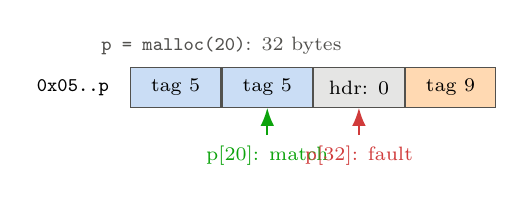
\begin{tikzpicture}[font=\scriptsize, cell/.style={draw=ink2, minimum width=1.15cm, minimum height=0.5cm}]
\node[cell, fill=accent!25] (a) {tag 5};
\node[cell, fill=accent!25, right=0pt of a] (b) {tag 5};
\node[cell, fill=ink2!15, right=0pt of b] (h) {hdr: 0};
\node[cell, fill=orange!30, right=0pt of h] (c) {tag 9};
\node[above=1pt of a.north east, ink2] {\texttt{p = malloc(20)}: 32 bytes};
\node[left=4pt of a, align=right] {\texttt{0x05..p}};
\draw[-{Latex}, okc, thick] (b.south) ++(0,-0.35) -- (b.south) node[pos=0, below, okc] {p[20]: match};
\draw[-{Latex}, badc, thick] (h.south) ++(0,-0.35) -- (h.south) node[pos=0, below, badc] {p[32]: fault};
\end{tikzpicture}
\end{frame}

\begin{frame}{Starting point: Noh et al.\ (USENIX Security 2026)}
\begin{itemize}\itemsep5pt
\item The paper measures Pixel 8/9 (Cortex-X, A7x, A5x), AmpereOne and Apple M5 on SPEC CPU, RocksDB, Nginx, PostgreSQL and Memcached.
\item Their setup, which we reproduce: Clang/GCC binaries and glibc 2.36, with MTE enabled via \texttt{glibc.mem.tagging} on the \emph{same binary}.
\item Overheads are often modest, but with cliffs:
\begin{itemize}\small
\item \textbf{6.64$\times$} (456.hmmer, Pixel Performance core, SYNC): store serialization
\item \textbf{1.82$\times$} even in ASYNC (Pixel Big core): tag-check structural hazard
\item 1.10$\times$ geomean on AmpereOne (SYNC); 1.43$\times$ from store-to-load forwarding
\end{itemize}
\item Tagging large allocations (\texttt{STG}) is a visible cost.
\end{itemize}
\take{They measure the cost; we measure what you get for it.}
\end{frame}

%---------------------------------------------------------------
\begin{frame}{Experimental setup}
\footnotesize
\begin{tabular}{@{}lll@{}}
\toprule
Config & How & Platform\\
\midrule
Baseline & \texttt{-fno-stack-protector -D\_FORTIFY\_SOURCE=0} & x86 + A64\\
Hardening & \texttt{-fstack-protector-strong -D\_FORTIFY\_SOURCE=3} & x86 + A64\\
 & \texttt{-fsanitize=bounds-strict -fsanitize-trap=all} & \\
ASan & \texttt{-fsanitize=address} & x86-64\\
MTE-sync & baseline binary + \texttt{glibc.mem.tagging=3} & A64\\
MTE-async & baseline binary + \texttt{glibc.mem.tagging=1} & A64\\
\bottomrule
\end{tabular}
\vspace{0pt}
\begin{itemize}\itemsep2pt
\item \textbf{x86-64}: Ryzen 5 5600H, native. Real timings for Baseline, Hardening and ASan.
\item \textbf{AArch64 + MTE}: QEMU 10.2 user mode, \texttt{-cpu max}. Functional MTE; timings reflect \emph{emulation}.
\item A fault reporter in every test logs signal, \texttt{si\_code} (sync 9 / async 8), address, PC $\rightarrow$ \texttt{file:line}.
\item Baseline/Hardening on \emph{both} platforms are controls: MTE vs.\ A64 baseline (same binary), ASan vs.\ x86 baseline.
\item Detection: 20 runs per (program, config), \textbf{1{,}400 runs}. Performance: median time and peak RSS (5 runs), \texttt{perf stat} on x86-64.
\end{itemize}
\end{frame}

\begin{frame}{Three methodology pitfalls we hit}
\begin{enumerate}\itemsep8pt
\item \textbf{The compiler deletes the bugs.} At \texttt{-O1}/\texttt{-O2}, GCC removes \texttt{malloc; free; p[0]=42} and dead-buffer \texttt{strcpy} as UB.\\
\hspace{1em}$\rightarrow$ The suite is built at \texttt{-O0} for every config.
\item \textbf{glibc 2.43's MTE is broken under QEMU.} \texttt{free()} raises a tag fault on \emph{every} call, so every run is a false positive.\\
\hspace{1em}$\rightarrow$ We use Debian's glibc \textbf{2.36}, the same version as the paper.
\item \textbf{ASan cannot run under QEMU user mode} (shadow reservation fails).\\
\hspace{1em}$\rightarrow$ ASan is run natively on x86-64.
\end{enumerate}
\end{frame}

%---------------------------------------------------------------
\begin{frame}{Phase 1: suite and boundary cases}
\small
\begin{columns}[T]
\column{0.47\textwidth}
\textbf{Suite} (proposal)
\begin{itemize}\itemsep2pt
\item stack overflow: 21 B into \texttt{char[10]}
\item heap overflow: 21 B into \texttt{malloc(10)}
\item OOB read / write: \texttt{arr[5]} of \texttt{int[5]}
\item use-after-free: write after \texttt{free}
\item double-free
\end{itemize}
\column{0.5\textwidth}
\textbf{Boundary cases} (RQ2)
\begin{itemize}\itemsep2pt
\item[B1] write byte 12 of \texttt{malloc(10)}: inside the granule
\item[B2] OOB index that jumps into another \emph{live} object
\item[B3] UAF after 320 MiB churn: chunk reused
\item[B4] overflow \texttt{name[16]} $\rightarrow$ function pointer in the same \texttt{struct}, then call it
\end{itemize}
\end{columns}
\end{frame}

\begin{frame}{RQ1/RQ2: detection matrix (observed, 20 runs per cell)}
\centering
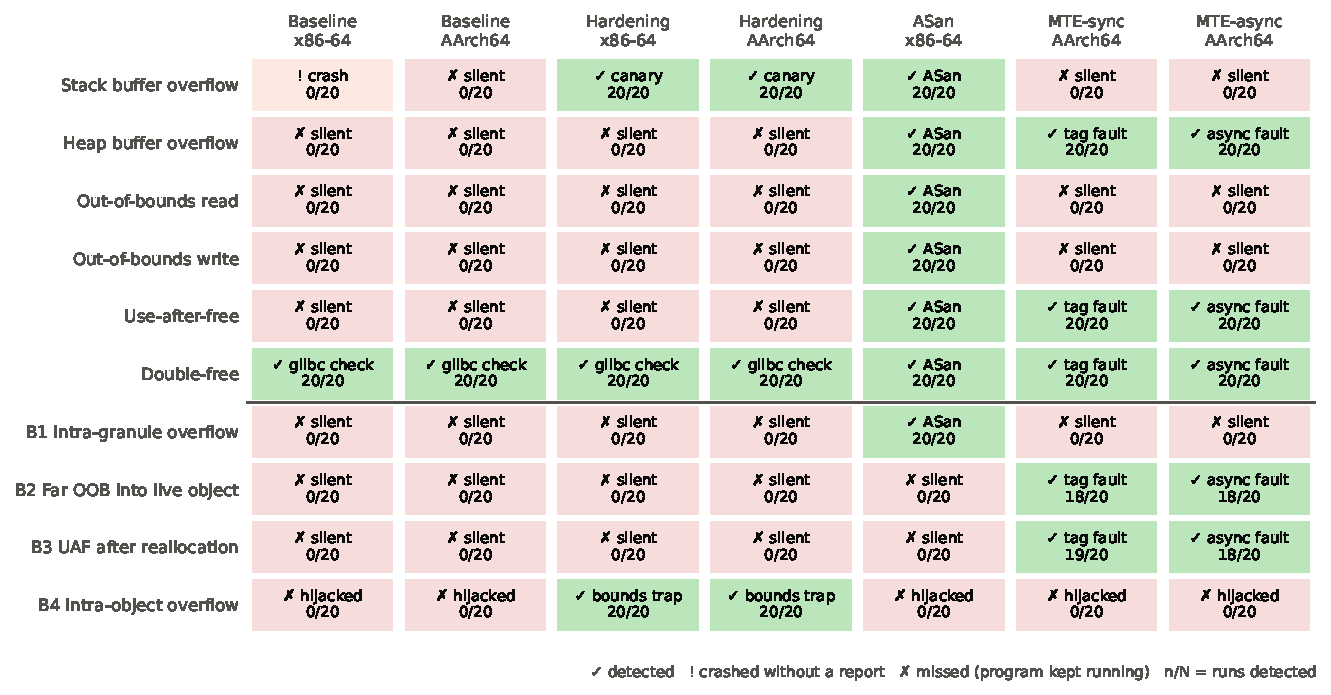
\includegraphics[width=0.93\textwidth]{../figures/detection_matrix.pdf}
\end{frame}

\begin{frame}{RQ1: coverage on the suite}
\begin{itemize}\itemsep6pt
\item \textbf{ASan: 6/6}, deterministic, exact line and bug class.
\item \textbf{MTE: 3/6}: heap overflow, UAF and double-free, with no recompilation.
\begin{itemize}\small
\item \xmark\ stack overflow: glibc tags only the heap; GCC has no stack tagging.
\item \xmark\ OOB read/write: \texttt{malloc(20)} is rounded to 32 B; \texttt{arr[5]} lies in the object's \emph{own} padding. \textbf{Deterministic miss.}
\end{itemize}
\item \textbf{Canary}: catches the stack overflow, but only at \texttt{return}, after the code has run on.
\item \textbf{Baseline}: glibc's tcache already catches the double-free; the x86 stack overflow only \emph{crashes}.
\end{itemize}
\take{MTE's spatial resolution is 16 bytes, not 1 byte.}
\end{frame}

\begin{frame}{RQ2: the mechanisms fail on \emph{different} bugs}
\begin{columns}[T]
\column{0.5\textwidth}
\small
\begin{tabular}{@{}lcc@{}}
\toprule
Case & ASan & MTE\\
\midrule
B1 intra-granule & \cmark\ 20/20 & \xmark\ 0/20\\
B2 far OOB, live obj & \xmark\ 0/20 & \cmark\ 18/20\\
B3 UAF after reuse & \xmark\ 0/20 & \cmark\ 19/20\\
B4 intra-object & \xmark & \xmark\\
\bottomrule
\end{tabular}
\vspace{6pt}
\begin{itemize}\small\itemsep2pt
\item B4 hijacks control flow in every run; only \texttt{-fsanitize=bounds-strict} traps it.
\item Memory tagging is \textbf{not} a CFI substitute (Topic 5).
\end{itemize}
\column{0.48\textwidth}
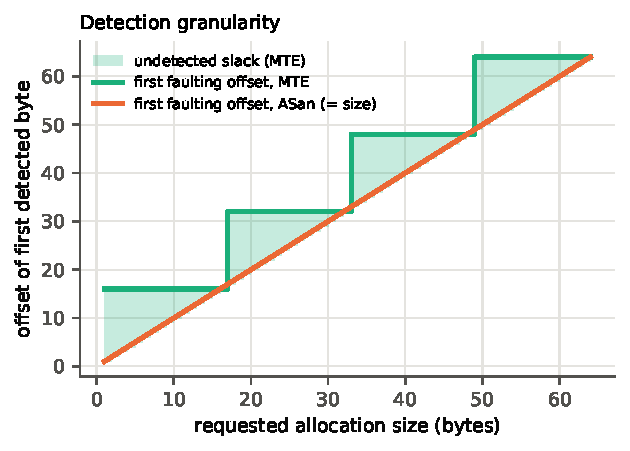
\includegraphics[width=\linewidth]{../figures/granule.pdf}
\end{columns}
\end{frame}

\begin{frame}{RQ3: synchronous vs.\ asynchronous MTE}
\small
Probe: one illegal store (or 16 illegal loads) into a neighbouring ``secret'' object, then a syscall-free loop.
\vspace{6pt}
\centering
\begin{tabular}{@{}llccc@{}}
\toprule
Access & Mode & fault address & store committed? & leaked bytes used\\
\midrule
store & SYNC & exact & no & --\\
store & ASYNC & \texttt{0} & \textbf{yes} & --\\
load & SYNC & exact & -- & 0\\
load & ASYNC & \texttt{0} & -- & \textbf{1}\\
\bottomrule
\end{tabular}
\raggedright
\begin{itemize}\itemsep3pt
\item Both modes detect the same suite bugs; ASYNC reports at the next library call (\texttt{puts@plt}).
\item On hardware the ASYNC report waits for the next \emph{kernel entry}: a longer window.
\item Emulated runtime: ASYNC $\approx$ \AsyncVsSync$\times$ SYNC. Not meaningful; the paper shows SYNC cliffs of up to 6.64$\times$.
\end{itemize}
\take{ASYNC detects after the fact; it does not prevent the write.}
\end{frame}

\begin{frame}{RQ4: native overhead (x86-64)}
\centering
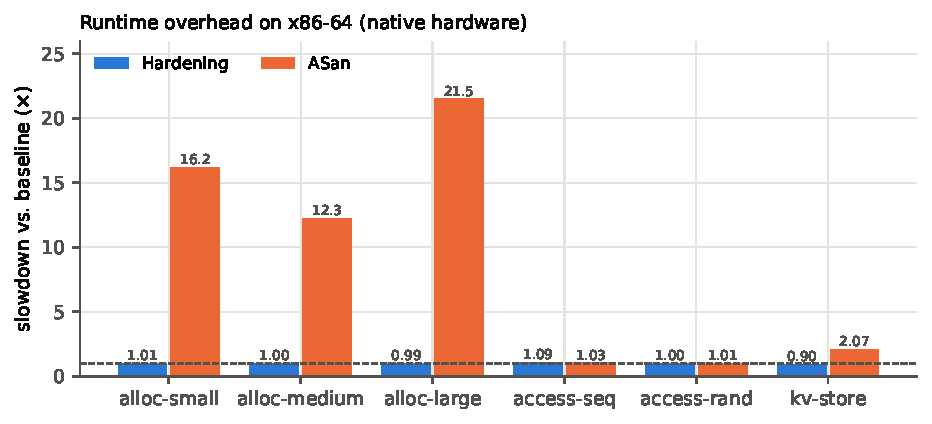
\includegraphics[height=0.39\textheight]{../figures/perf_x86.pdf}\\
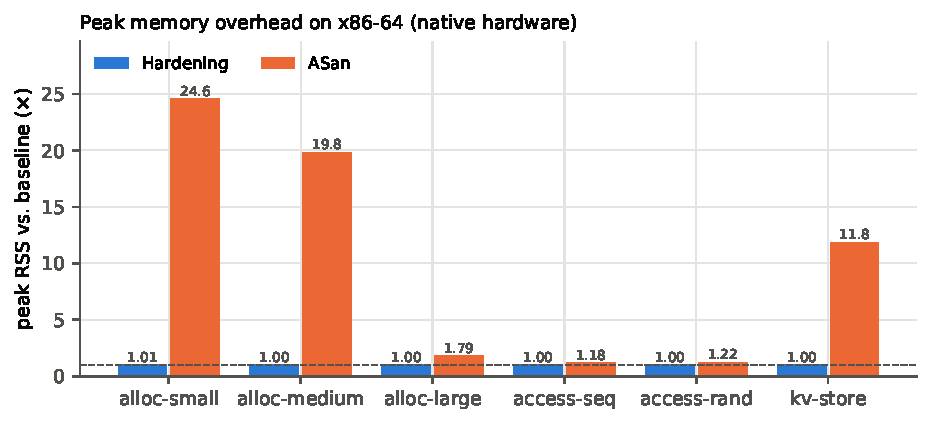
\includegraphics[height=0.39\textheight]{../figures/perf_x86_rss.pdf}\\[-2pt]
\raggedright\small ASan cost is driven by allocation (redzones, poisoning, quarantine), not by checking each access: memory-bound loops cost only $\approx$1.0$\times$.
\end{frame}

\begin{frame}{RQ4: why ASan costs what it costs (\texttt{perf stat}, x86-64)}
\centering\scriptsize
\CounterTable
\vspace{8pt}
\raggedright\small
\begin{itemize}\itemsep2pt
\item \textbf{Allocation-heavy:} up to \AsanSmallInstr$\times$ instructions, \AsanSmallPf$\times$ page faults, IPC drops (\BaseLargeIpc$\to$\AsanLargeIpc): quarantine and shadow poisoning are memory traffic.
\item \textbf{Memory-bound:} \AsanSeqInstr$\times$ instructions but \AsanSeqCyc$\times$ cycles: shadow checks hide behind DRAM stalls.
\item \textbf{Hardening:} \HardInstrMin--\HardInstrMax$\times$ instructions; its timing differences are noise.
\end{itemize}
\end{frame}

\begin{frame}{RQ4: AArch64 under QEMU: where MTE adds work}
\centering
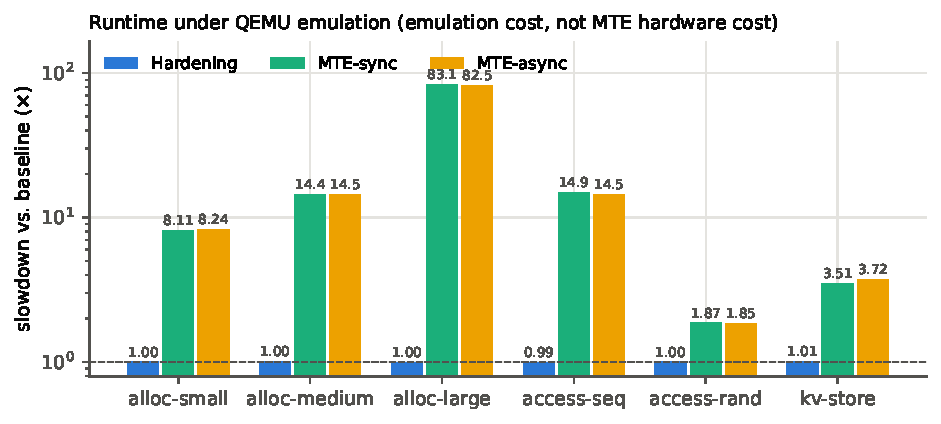
\includegraphics[width=0.85\textwidth]{../figures/perf_qemu.pdf}
\raggedright\small
\begin{itemize}\itemsep2pt
\item This is emulation cost: QEMU checks tags in software.
\item The relative pattern is still informative: cost grows with \textbf{bytes tagged per allocation} (\texttt{STG} on every \texttt{malloc}/\texttt{free}), matching the paper's large-allocation finding (\S4.4.4).
\end{itemize}
\end{frame}

%---------------------------------------------------------------
\begin{frame}{Phase 4: the finite tag space, detection vs.\ distance}
\centering
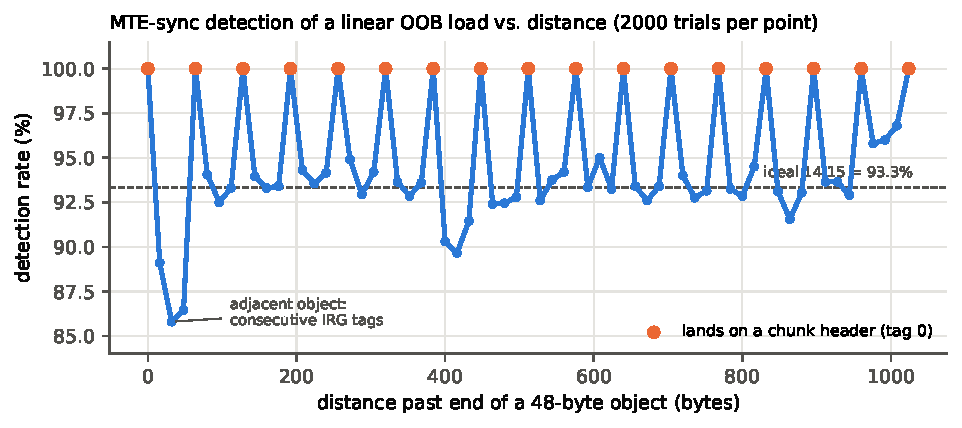
\includegraphics[width=0.9\textwidth]{../figures/tag_distance.pdf}
\raggedright\small
\begin{itemize}\itemsep2pt
\item Chunk headers carry tag 0 (never assigned to user pointers): \textbf{100\%}.
\item Far objects: \textbf{\FarMean\%}, close to the ideal 14/15.
\item Adjacent object: only \textbf{\AdjMin--\AdjMax\%}.
\end{itemize}
\end{frame}

\begin{frame}{Phase 4: accidental tag matches after reuse}
\begin{columns}[T]
\column{0.52\textwidth}
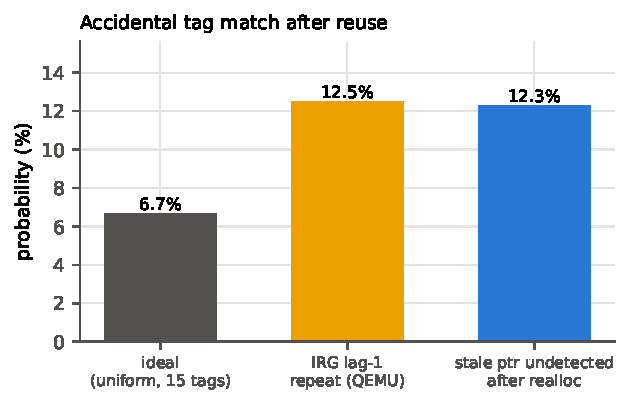
\includegraphics[width=\linewidth]{../figures/tag_reuse.pdf}
\column{0.46\textwidth}
\small
\begin{itemize}\itemsep4pt
\item Freed memory is re-tagged to 0, so UAF before reuse: 100\% detected.
\item After reallocation: \textbf{\ReuseUndet\%} undetected (\ReuseTrials\ trials), against 6.7\% ideal.
\item Cause: consecutive \texttt{IRG} tags repeat \textbf{\IrgLagOne\%} of the time in QEMU.
\item The same correlation explains the weak adjacent-object rate.
\end{itemize}
\take{The guarantee is only as good as the tag generator.}
\end{columns}
\end{frame}

%---------------------------------------------------------------
\begin{frame}{Security--performance trade-off}
\footnotesize
\begin{tabular}{@{}p{1.9cm}p{3.9cm}p{3.7cm}p{3.2cm}@{}}
\toprule
 & Detects & Misses & Cost\\
\midrule
Hardening & stack smash (at return), index OOB & all heap bugs & $\approx$1.0$\times$\\
ASan & all 6 suite bugs, byte-precise & far OOB, UAF after quarantine & \AsanMin--\AsanMax$\times$ time, up to \AsanRssMax$\times$ RSS\\
MTE-sync & heap OOB beyond granule, UAF, double-free, far OOB, reuse & stack, sub-granule, intra-object & 3.1\% tag storage; hw: modest + cliffs\\
MTE-async & same, \emph{after} the access & + no address & cheaper on hw (paper)\\
\bottomrule
\end{tabular}
\vspace{8pt}
\begin{itemize}\itemsep3pt
\item The mechanisms are \textbf{complementary}: ASan for testing, MTE for production, plus stack protection and CFI.
\end{itemize}
\end{frame}

\begin{frame}{Course mapping, limitations, conclusion}
\small
\begin{columns}[T]
\column{0.48\textwidth}
\textbf{Course topics}
\begin{itemize}\itemsep2pt
\item T1--2: stack smashing, the suite
\item T3: software vs.\ hardware defenses
\item T4: redzones/shadow vs.\ 16-byte tags
\item T5: B4 shows MTE $\neq$ CFI
\item T16: MTE instructions, modes, glibc/kernel integration
\end{itemize}
\textbf{Limitations}
\begin{itemize}\itemsep2pt
\item No MTE silicon: QEMU validates behaviour, not timing
\item ASan on x86-64; no stack tagging (GCC); ASYMM not evaluated
\end{itemize}
\column{0.5\textwidth}
\textbf{Conclusion}
\begin{itemize}\itemsep4pt
\item ASan: deterministic, byte-precise, too costly for production.
\item MTE: no recompilation; catches the long-range and temporal bugs ASan misses, probabilistically and at 16-byte resolution.
\item ASYNC trades prevention for detection.
\item Neither stops an intra-object control-flow hijack.
\end{itemize}
\end{columns}
\end{frame}

\begin{frame}
\centering\Huge Thank you\\[10pt]
\normalsize Questions?\\[16pt]
\small\color{ink2} All code, data and scripts: \texttt{memory-safety-eval} repository (\texttt{./run\_all.sh})
\end{frame}

\end{document}
